\chapter{L1 Trigger Data Quality Monitoring}
\label{CHAPTER:TechnicalWork}

% \glsresetall % Resetting all acronyms

% Status: DONE (reviewed J.Pela x1) (reviewed D. Colling x1)

The \gls{CMS} \gls{L1T} makes the first event selection of any physics analysis. Therefore, its correct operation is crucially for the physics output of the experiment. The \gls{DQM} is one of the \gls{CMS} monitoring systems which is able to provide both real-time monitoring and offline analysis of the detector operation. This chapter describes the \gls{L1T} \gls{DQM} applications developed and used for online monitoring and data certification for physics analyses of the during 2012-13 data taking.

%%%%%%%%%%%%%%%%%%%%%%%%%%%%%%%%%%%%%%%%%%%%%%%%%%%%%%%%%%%%%%%%%%%%%%%%%%%%%%%%%%%%%%%
%%% SECTION
%%%%%%%%%%%%%%%%%%%%%%%%%%%%%%%%%%%%%%%%%%%%%%%%%%%%%%%%%%%%%%%%%%%%%%%%%%%%%%%%%%%%%%%
\section{Data Quality Monitoring}
\label{SECTION:TechnicalWork_DataQualityMonitoring}

% Status: DONE (reviewed J.Pela x1) (reviewed D. Colling x1)

The \gls{DQM} is a critical monitoring system that has an important role in detector and operations efficiency. It also important in the certification of recorded data for physics analysis \cite{CMSTDR:CMSTridasTDRVol1,ARTICLE:CMSDataQualityMonitoringSoftWare_ExperienceAndFuture}. The \gls{DQM} system is an end-to-end solution that provides tools to create, fill, display and archive histograms and scalar monitors. It provided the ability to monitor the detector and \gls{DAQ} in real-time, analyse the reconstruction process, validate the experiment's software releases and its simulated data. The purpose of this system is to identify problems or errors in both hardware and software as early and accurately as possible.

%%%%%%%%%%%%%%%%%%%%%%%%%%%%%%%%%%%%%%%%%%%%%%%%%%%%%%%%%%%%%%%%%%%%%%%%%%%%%%%%%%%%%%%
%%% SUBSECTION
%%%%%%%%%%%%%%%%%%%%%%%%%%%%%%%%%%%%%%%%%%%%%%%%%%%%%%%%%%%%%%%%%%%%%%%%%%%%%%%%%%%%%%%
\subsection{Online Monitoring}
\label{SECTION:TechnicalWork_DataQualityMonitoring_OnlineMonitoring}

% Status: DONE (reviewed J.Pela x1) (reviewed D. Colling x1)

The online \gls{DQM} system is composed of several applications that are part of the \gls{CMS} data processing work flow. The software is executed on the \gls{CMS} computing cluster at point 5. Applications fall into two categories: \textit{high level trigger modules} and \textit{data quality monitoring modules}. The \textit{high level trigger modules} are run directly on the \gls{HLT} filter farm and can only produce a limited number of histograms which of monitor that system or specific \gls{HLT} path. The \textit{data quality monitoring modules} run over events coming from a dedicated \gls{DQM} event stream with a rate of $5-10\,\hertz$. These events contain only the raw detector and trigger information. Each subsystem has its own application which can analyse all events from the stream or filter a subset with a predefined trigger selection. At the end of every luminosity section, which corresponds to $23.31\,\second$, histograms are gathered from the nodes where the applications are run and are merged together. The results are showed in real time in a web based application which is accessible by the shift crew and on call experts.

%%%%%%%%%%%%%%%%%%%%%%%%%%%%%%%%%%%%%%%%%%%%%%%%%%%%%%%%%%%%%%%%%%%%%%%%%%%%%%%%%%%%%%%
%%% SUBSECTION
%%%%%%%%%%%%%%%%%%%%%%%%%%%%%%%%%%%%%%%%%%%%%%%%%%%%%%%%%%%%%%%%%%%%%%%%%%%%%%%%%%%%%%%
\subsection{Offline Monitoring}
\label{SECTION:TechnicalWork_DataQualityMonitoring_OfflineMonitoring}

% Status: DONE (reviewed J.Pela x1) (reviewed D. Colling x1)

The offline \gls{DQM} is used in numerous workflows including monitoring of the event reconstruction process, alignment and calibration validation, \gls{CMS} software release validation, etc. For all these tasks a standardized two step process is run. 

In the first step histograms are produced in the same computing jobs of the task to be monitored and stored along with the rest of the event data. This is happens in multiple simultaneous jobs which depending on the task can be at Tier 0 or Tier 1 level.

In the second, \textit{harvesting step}, the histograms are extracted from the event data and summed together. The resulting histograms contain the full event yields from each run for each processed dataset. Applications running at this step have access to the detector conditions from the \gls{DCS} and the \gls{DAQ} and can produce new histograms like summaries of the relevant quantities for each run.

%%%%%%%%%%%%%%%%%%%%%%%%%%%%%%%%%%%%%%%%%%%%%%%%%%%%%%%%%%%%%%%%%%%%%%%%%%%%%%%%%%%%%%%
%%% SECTION
%%%%%%%%%%%%%%%%%%%%%%%%%%%%%%%%%%%%%%%%%%%%%%%%%%%%%%%%%%%%%%%%%%%%%%%%%%%%%%%%%%%%%%%
\section{Level 1 Trigger Data Quality Monitoring}
\label{SECTION:TechnicalWork_L1TDQM}

% Status: DONE (reviewed J.Pela x1) (reviewed D. Colling x1)

The \gls{L1T} \gls{DQM} is composed of four applications. The first two application run as part of the online \gls{DQM} system and monitor the trigger hardware and emulation in real-time. The second pair of applications runs in the offline \gls{DQM} system as part of the (re-)reconstruction workflow with and provide information for physics data certification.

The first of the two online applications directly monitors the operation of the trigger. Each trigger subsystem produces plots of its own relevant quantities including information which allows it to pin-point the origin of problems. Additionally, a set of monitoring tools observe the final objects and global behaviour of the system. Key aspects are analysed such as the value of reference algorithm rates, synchronization of firing, finding regions of the detector that show unexpected high/low rate. 

The second online application compares the results of the trigger against a real-time software emulation of the system which should allow quick detection of trigger miss configuration or degradation of quality of operation.

Both offline monitoring applications replicate the analysis preformed by their online counterparts but over a the complete recorded dataset for each run.

In the next sections we will focus on the trigger monitoring tools that the author developed or significantly improved.

%%%%%%%%%%%%%%%%%%%%%%%%%%%%%%%%%%%%%%%%%%%%%%%%%%%%%%%%%%%%%%%%%%%%%%%%%%%%%%%%%%%%%%%
%%% SUBSECTION
%%%%%%%%%%%%%%%%%%%%%%%%%%%%%%%%%%%%%%%%%%%%%%%%%%%%%%%%%%%%%%%%%%%%%%%%%%%%%%%%%%%%%%%
\subsection{Rates Monitoring}
\label{SECTION:TechnicalWork_L1TDQM_RatesMonitoring}

% Status: DONE (reviewed J.Pela x1)

The rates monitoring tool has the objective of inspecting the firing rate of each \gls{L1T} object category. At the beginning of each run the \gls{L1T} menu is analysed and for each object category the lowest thresholds unprescaled algorithm is selected. If no unprescaled algorithm is available the lowest prescale and threshold trigger is selected. If the selected trigger algorithms are $\eta$ restricted a warning is showed in the produced histograms to identify that the tests performed do not cover the full acceptance of the monitored object. The following categories of objects can be monitored: Electron-Gamma, Isolated Electron-Gamma, Central Jets ($|\eta|<3$), Forward Jets ($3<|\eta|<5$), All Jets ($|\eta|<5$), Taus, Muon, total energy (ETT), total energy in jets (HTT), missing energy (ETM) and jets missing energy (HTM).

When the algorithms to be monitored are determined the tool retrieves from an external database the expected algorithm cross section as a function of the instantaneous luminosity. These functions are updated daily by fitting runs from the previous days with similar condition. This task is executed by the \gls{WbM} which is a \gls{CMS} monitoring system which runs in parallel to the \gls{DQM}. The algorithm cross section for each luminosity section is calculated with following equation \ref{EQUATION:TechnicalWork_AlgoCrossSection}.

\begin{equation}
\sigma_{\text{Algo}}=\frac{\text{Prescale}_{\text{Algo}}*{\text{Avg. Rate}_{\text{Algo}}}}{\text{Avg. Instantaneous Luminosity}*(1-\text{CMS Dead time fraction})}
\label{EQUATION:TechnicalWork_AlgoCrossSection}
\end{equation}

The measured value is compared with prediction from previous runs for each luminosity section. The monitor presents this results in histograms with the measured value and the relative value to prediction. An example of this histograms can be found in figure \ref{FIGURE:TechnicalWork_RateMonitoring}

\begin{figure}[!htb]
\centering
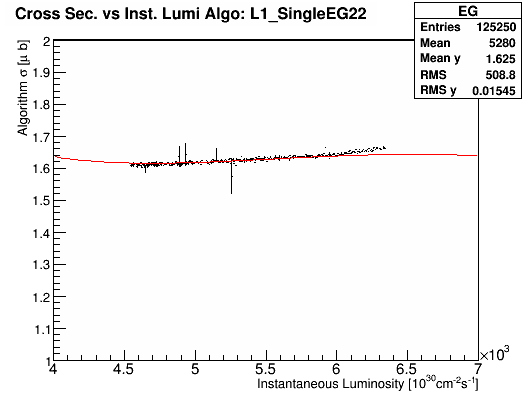
\includegraphics[width=0.45\textwidth]{Chapter03/L1TOnline/Images/L1TDQM_Online_Run207269_L1TRate_TriggerCrossSections_EG.png}
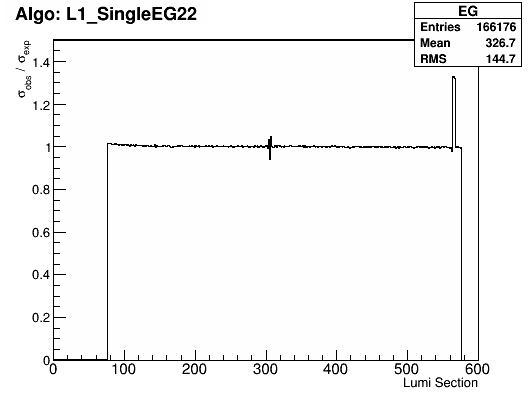
\includegraphics[width=0.45\textwidth]{Chapter03/L1TOnline/Images/L1TDQM_Online_Run207269_L1TRate_Certification_EG.png}
\caption{Monitoring plots produced by the \gls{L1T} online rates monitoring tool for run 207269 and the Electron-Gamma object category. The automatically selected algorithm was L1\_SingleEG22 for this run. On the left histogram  the algorithm cross section as a function of instantaneous luminosity is plotted. The red line is the prediction obtained from fitting data from previous runs while the black points are the measurements for this run. On the right histogram the fraction of the measured value over the prediction is showed as a function of the luminosity section.}
\label{FIGURE:TechnicalWork_RateMonitoring}
\end{figure}

Automatic tests are configured to monitor the produced histograms and flag as bad the luminosity sections that show deviation from prediction above 20\%. Marking a specific luminosity section as bad does not invalidate its use for physics analysis, but references it for further investigation by the \gls{CMS} shift crew or certification experts.

%%%%%%%%%%%%%%%%%%%%%%%%%%%%%%%%%%%%%%%%%%%%%%%%%%%%%%%%%%%%%%%%%%%%%%%%%%%%%%%%%%%%%%%
%%% SUBSECTION
%%%%%%%%%%%%%%%%%%%%%%%%%%%%%%%%%%%%%%%%%%%%%%%%%%%%%%%%%%%%%%%%%%%%%%%%%%%%%%%%%%%%%%%
\subsection{Synchronization Monitoring}
\label{SECTION:TechnicalWork_L1TDQM_SynchronizationMonitoring}

% Status: DONE (reviewed J.Pela x1)

The synchronization monitoring tool has the objective of assessing if each \gls{L1T} object category is being produced and associated with the correct bunch crossing. Similarly to the \gls{L1T} rates monitoring tool described in the previous section, in the beginning of each run we select the lowest thresholds unprescaled algorithm for each object category. If none are available the algorithm with lowest prescale and lowest threshold is selected.

The information of which bunch crossings are filled is retrieved at the beginning of each run by \gls{CMS}. That information is stored in a database at point 5 and later replicated to the \gls{CMS} offline conditions database. At the same time, the synchronization monitoring tool determines the \gls{LHC} fill number from the \gls{L1T} \gls{GT} system. Data from the \gls{LHC} is obtained via the \gls{DIP} which allows exchange of information between detect and accelerator. With this information the bunch crossing information is retrieved from the \gls{OMDS} when running online and from \gls{ORCON} when running offline.

When selected events are desynchronized from the correct bunch crossing at the \gls{L1T} level, these events will appear empty from the \gls{HLT} and offline perspectives. Therefore it is unlikely that they will pass any \gls{HLT} triggers, making it very difficult to spot this type off problems. For this reason the synchronization monitoring looks only at events that come from special \gls{HLT} trigger, the \gls{HLT} pass-through paths. These triggers are highly prescaled and only required that a specific \gls{L1T} condition is fired. All available \gls{HLT} pass-through paths of single object \gls{L1T} trigger are monitored by this tool.

All events triggered passing \gls{HLT} pass-through paths are analysed and all selected algorithms firing is compared to the actual \gls{LHC} bunch crossing filling and the results are recorded. Additionally, for each event we query the \gls{GT} about the \gls{LHC} beam mode and if for any event the status is not \text{Stable Beams}, the luminosity section is immediately marked as bad.

Since we are running this monitoring only over the events that pass \gls{HLT} pass-through paths a single luminosity section will typically not have enough statistics to take conclusions on the behaviour of the system. To provide reliable results at the end of each luminosity section it is decided if the current luminosity section has enough statistics by itself of needs to be grouped with the previous ones. Blocks of luminosity section are made until a minimum configurable number of events is reached for each individual monitored trigger. At this point the histogram of the fraction of events in time with bunch crossings is updated. If the \gls{LHC} beam mode changes or the the run ends, the current open luminosity sections block is closed with the current statistics. The histograms produced by this tool for run 207269 can be found in figure \ref{FIGURE:TechnicalWork_SyncMonitoring}.

\begin{figure}[!htb]
\centering
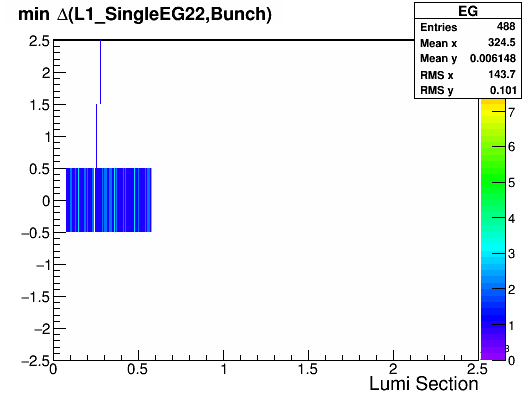
\includegraphics[width=0.45\textwidth]{Chapter03/L1TOnline/Images/L1TDQM_Online_Run207269_L1TSync_AlgoVsBunchStructure_EG.png}
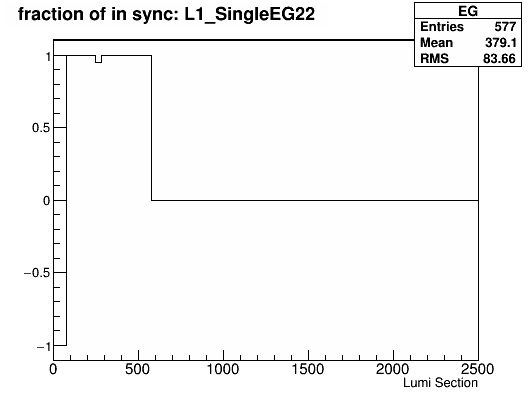
\includegraphics[width=0.45\textwidth]{Chapter03/L1TOnline/Images/L1TDQM_Online_Run207269_L1TSync_Certification_EG.png}
\caption{Monitoring plot produced by the L1TSync tool for L1 single electron/gamma object category, which is
automatically monitoring algorithm L1\_SingleEG22 for the run 207269. In the plots data points are the calculated
trigger cross section as a function of instant luminosity and the line is the reference fit done from previous runs.}
\label{FIGURE:TechnicalWork_SyncMonitoring}
\end{figure}

Similarly to the \gls{L1T} rates monitoring tool, automatic tests are configured to flag as bad luminosity sections that show deviation from prediction above 20\%. 

%%%%%%%%%%%%%%%%%%%%%%%%%%%%%%%%%%%%%%%%%%%%%%%%%%%%%%%%%%%%%%%%%%%%%%%%%%%%%%%%%%%%%%%
%%% SUBSECTION
%%%%%%%%%%%%%%%%%%%%%%%%%%%%%%%%%%%%%%%%%%%%%%%%%%%%%%%%%%%%%%%%%%%%%%%%%%%%%%%%%%%%%%%
\subsection{BPTX Monitoring}

% Status: DONE (reviewed J.Pela x1)

The \gls{BPTX} system is composed of two beam detectors located in each beam pipe $175\,\meter$ upstream of the \gls{CMS} experiment \cite{ARTICLE:TheCMSExperiment}. This detectors were designed to provide precise information about the bunch structure and timing of each beam and have sensitivity to time structures under $25\,\nano\second$. 

In early 2012 a problem was identified in the \gls{L1T} where some events would fire on the bunch crossing before the actual event. It was discovered that this effect was most likely connect to sensors in the calorimeter system being directly hit by particles causing a large out-of-time signal. Unfortunately, the trigger has a set of rules intended to limit the event rate. They are necessary in order to allow for the necessary latency to extract the information from the detector in case a collision is accepted. One of these rules states that if a collision is accepted by the \gls{L1T} the next 2 collisions are ignore by the system \cite{CMSTDR:CMSTridasTDRVol1}. This means that if a specific event causes the \gls{L1T} to fire on the previous bunch crossing, that event will be vetoed by trigger rules. To avoid losing interesting events due to this pre-firing problem the signal of both \gls{BPTX} detectors logical AND was advanced by one bunch crossing and connected to the trigger via a technical algorithm bit. This bit in turn was used to veto the \gls{L1T} from firing.

Although this was a successful solution to this problem it caused preoccupation in the \gls{TSG} and \gls{L1T} \gls{DPG} groups. Since if the \gls{BPTX} bunch detection threshold would be set too high this veto would be ineffective, leading to no bunches being detect and no veto being applied. If the \gls{BPTX} bunch detection threshold would be set too low, residual amounts of protons or noise in the unfilled bunch spaces could lead to vetoing filled bunch spaces. The development and commissioning of a monitoring tool was requested as priority task.

A new tool was developed to compare the \gls{LHC} filling scheme with the firing of the technical trigger associated with the \gls{L1T} veto. Following the ideas of the \gls{L1T} synchronization monitoring tool the same procedure was used to retrieve the \gls{LHC} filling scheme and algorithm firing results. For each selected event the \gls{GT} records the results of each \gls{L1T} trigger algorithm for the two previous and two posterior bunch crossings. For this tool all five recorded bunch crossings in each event are compares with the \gls{LHC} bunch structure. In this case we are interested in both efficiency, since low efficiency would mean that the \gls{BPTX} bunch detection threshold would be too low. And miss fire rate, which would be associated with a \gls{BPTX} bunch detection threshold would being too high. Examples of the histograms produced by this tool can be found in figure \ref{FIGURE:TechnicalWork_BPTXMonitoring}.

\begin{figure}[!htb]
\centering
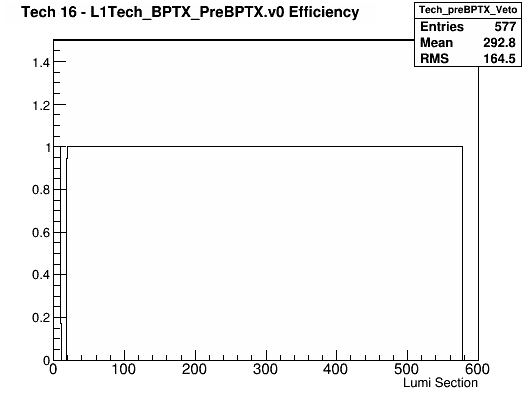
\includegraphics[width=0.45\textwidth]{Chapter03/L1TOnline/Images/L1TDQM_Online_Run207269_L1TBPTX_Efficiency_Tech_preBPTX_Veto.png}
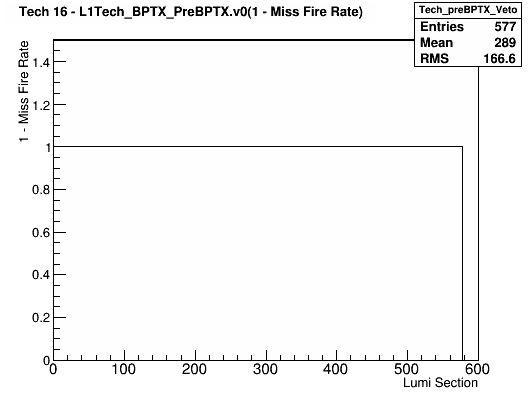
\includegraphics[width=0.45\textwidth]{Chapter03/L1TOnline/Images/L1TDQM_Online_Run207269_L1TBPTX_MissFire_Tech_preBPTX_Veto.png}
\caption{Monitoring plot produced by the \gls{L1T} \gls{BPTX} monitoring tool for \gls{CMS} run 207269. On the left the \gls{BPTX} veto efficiency in relation to the \gls{LHC} fill bunch structure is showed. On the right for the same algorithm $1 - \text{Miss Fire fraction}$ is showed.}
\label{FIGURE:TechnicalWork_BPTXMonitoring}
\end{figure}

%%%%%%%%%%%%%%%%%%%%%%%%%%%%%%%%%%%%%%%%%%%%%%%%%%%%%%%%%%%%%%%%%%%%%%%%%%%%%%%%%%%%%%%
%%% SUBSUBSECTION
%%%%%%%%%%%%%%%%%%%%%%%%%%%%%%%%%%%%%%%%%%%%%%%%%%%%%%%%%%%%%%%%%%%%%%%%%%%%%%%%%%%%%%%
\subsubsection{Implementation Tests}

% Status: DONE (reviewed J.Pela x1)

To test that the \gls{BPTX} monitoring tool would be successful in detecting the possible failure of the \gls{BPTX} system a field test was necessary. During run 207269 in which real data recorded the author with the permission of the \gls{L1T} \gls{DPG} disabled the technical \gls{L1T} bit associated with the \gls{BPTX} AND signal advanced by one luminosity section which was configured as a veto in the system. The bit was kept disable for a few luminosity sections which was promptly identified by the monitoring tool as it can be seen in figure \ref{FIGURE:TechnicalWork_L1TBPTX_ImplementationTests}.

\begin{figure}[!htb]
\centering
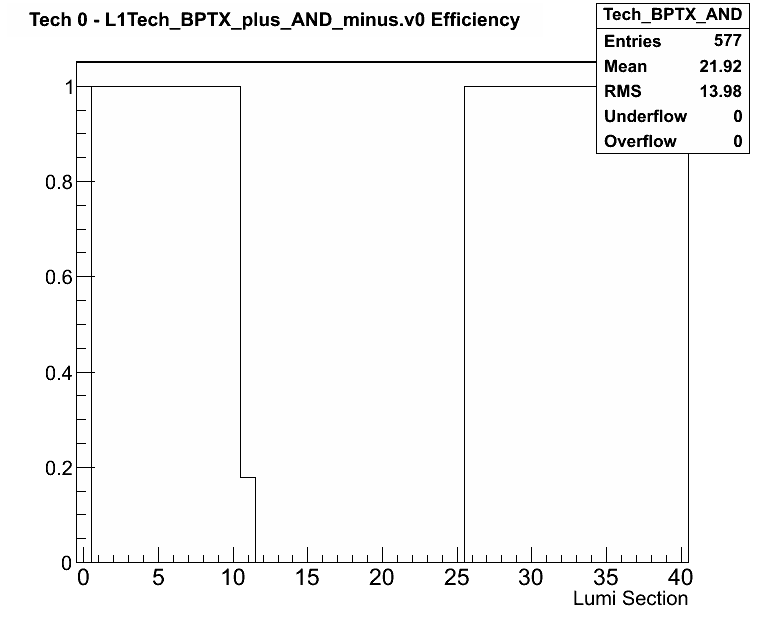
\includegraphics[width=0.45\textwidth]{Chapter03/L1TOnline/Images/L1TBPTX_Tech_BPTX_AND.png}
\caption{Detail of \gls{L1T} \gls{BPTX} monitoring tool histogram for veto efficiency during its field test at run 207269. The monitored bit was disabled manually leading to the monitored drop off efficiency.} 
\label{FIGURE:TechnicalWork_L1TBPTX_ImplementationTests}
\end{figure}

After this successful test the trigger shifter instruction were updated to include this histogram in the periodic checks to be done.  

%%%%%%%%%%%%%%%%%%%%%%%%%%%%%%%%%%%%%%%%%%%%%%%%%%%%%%%%%%%%%%%%%%%%%%%%%%%%%%%%%%%%%%%
%%% SUBSECTION
%%%%%%%%%%%%%%%%%%%%%%%%%%%%%%%%%%%%%%%%%%%%%%%%%%%%%%%%%%%%%%%%%%%%%%%%%%%%%%%%%%%%%%%
\subsection{Occupancy Monitoring}

% Status: DONE (reviewed J.Pela x1)

The occupancy monitoring tools objective is to identify regions of detector where the trigger system response has degraded. A region is considered \textit{dead} if the number measurements is null or its rate is consistently smaller than what would be expected for that area. Alternatively, a region can become \textit{hot} if the measurements rate is consistently bigger than expected for that area. This tool aims at identifying both of these categories of problems by analysis histograms produced by the trigger subsystems.

The main idea behind these tool is to use the $\eta$ and $\phi$ symmetries of the physics processes and experimental design. The collisions in \gls{CMS} happen in the centre of the experiment with beams of the same energy colliding head-on. Additionally, the detector is symmetric to the beam lines transverse plane passing on the collision point and also to the beam line itself. Both this factors imply that the response in a strip of cells across $\phi$ at constant $\eta$ should be the same on average in every cell and that response should be equivalent in a similar strip and constant $-\eta$.

The test consists of initially selecting an histogram of a quantity that is expressed in absolute event counts per region and that exhibits the described $\eta$ and $\phi$ symmetries. The histogram is integrated for as many luminosity sections as necessary to have enough statistics for conclusive results. When enough statistics are gathered and starting from the centre, a strip of cells is defined along $\phi$ to one side of that symmetry line. The value of the median of the selected cells is determined. Each cell of the opposing strip is compare to this median with statistical tests tuned to detect significant deviations. If any tests are failed, the cell is marked as bad for the period of the histogram integration. We repeat the same procedure reversing the role of both strips. After all cells in the first strip pair is tested we move to the next two strips of cells in increasing $\eta$ and repeat the procedure until all cells in the histogram have been tested. For histograms where the symmetry line fall in the middle of a strip of cell, that strip is tested against itself. The median is used to avoid bias from outliers like the \textit{hot} or \textit{dead} cells we are aiming to identify. 

Cells which are already known to be problematic can be masked from this tool to avoid being always marked as bad and contributing to the calculation of the fraction of problematic cells.

%%%%%%%%%%%%%%%%%%%%%%%%%%%%%%%%%%%%%%%%%%%%%%%%%%%%%%%%%%%%%%%%%%%%%%%%%%%%%%%%%%%%%%%
%%% SUBSUBSECTION
%%%%%%%%%%%%%%%%%%%%%%%%%%%%%%%%%%%%%%%%%%%%%%%%%%%%%%%%%%%%%%%%%%%%%%%%%%%%%%%%%%%%%%%
\subsubsection{Statistical hypotheses test}

% Status: DONE (reviewed J.Pela x1)

Since we are analysing histograms of absolute number of entries, like the location on \gls{L1T} Electron-Gamma candidates, each cell will follow Poisson statistics \cite{BOOK:AppliedStatisticsAndProbabilityforEngineers}. The probability of obtaining an histogram cell with value $x$ when the expected value is $\mu$ is expressed in equation \ref{EQUATION:TechnicalWork_Occupancy_Poisson}.

\begin{equation}
P(x;\mu)=\frac{exp(-\mu) \cdot \mu^{x}}{x!}
\label{EQUATION:TechnicalWork_Occupancy_Poisson}
\end{equation}

The implemented statistical tests will evaluate each cell over two hypotheses. The null hypothesis $H_0$, considers that the cell is behaving as expected and that the average number of events is $\mu_0$. The alternative hypothesis $H_1$, proposes that this is a problematic cell with an average number of events of $\mu_1$. We can now define a test statistic $T$ as the log-likelihood ratio of the two hypothesis as defined in equation \ref{EQUATION:TechnicalWork_Occupancy_LogLikelihoodRatio}.

\begin{equation}
T=\ln\frac{P(x,\mu_1)}{P(x,\mu_0)}
\label{EQUATION:TechnicalWork_Occupancy_LogLikelihoodRatio}
\end{equation}

The test statistic $D=2 \cdot T$ will be $\chi^2$-distributed on the limit of infinite sample size. Two tests need to be preformed for the \textit{dead} and \textit{hot} hypotheses. The relationship between between $\mu_0$ and $\mu_1$ for both tests can be defined as $\mu_1=f \cdot \mu_0$ where $f$ is the factional deviation from $\mu_0$ to flag a cell as bad. The following values were chosen, for \textit{dead} cells $\mu_{\text{dead}}=f_{\text{dead}} \cdot \mu_0$ with $f_{\text{dead}}=0.1$ and $\mu_{\text{dead}}=f_{\text{dead}} \cdot \mu_0$ with $f_{\text{hot}}=2.0$ for \textit{hot} cells.

A test efficiency of $99\%$ with a fake rate of $1\%$ were chosen as key parameters to constrain the the test behaviour, where efficiency is the probability of correctly identifying a problematic cell and fake rate is the probability of marking one or more cells as bad in a single histogram. The choice of these parameters defines the test threshold $T_{\text{crit}}$ and implies a requirement on the minimum average number of events per cell depending on the number of bins per histogram.

If the test statistic $T$ is above the critical value $T_{\text{crit}}$ we reject $H_0$ and consider the cell as bad, if is it below $T_{\text{crit}}$ we do not reject $H_0$ and consider the cell as good. The critical value is set by a choice of confidence level of finding a problematic cell and depends on $\mu_0$. To determine $T_{\text{crit}}(Dead Cell)$ and $T_{\text{crit}}(Hot Cell)$ as a function of $\mu_0$ two sets \gls{MC} toy experiments were made. For each experiment, the variable $\mu_0$ was set between 0 and 1000, which is its typical range in the histograms to be monitor, and $\mu_1$ was set according to which bad cell hypothesis. For each experiment 500 value were determined around $\mu_1$ with poison distribution for which the test statistic $T$ was determined. The critical value for 99\% efficiency is the value of 0.01-\textit{percentile} of $T$ distribution. The results obtained for $T_{\text{crit}}$ were fit with second order polynomial as a function of $\mu_0$ (eq. \ref{EQUATION:TechnicalWork_Occupancy_Chi2Fits}).

\begin{equation}
T_{\text{crit}}=a \cdot \mu_0^2 + b \cdot \mu_0 + c
\label{EQUATION:TechnicalWork_Occupancy_Chi2Fits}
\end{equation}

The results of the determination of each $T_{\text{crit}}$ for each set of toys for both bad cell hypothesis and the corresponding fits can be found on figure \ref{FIGURE:TechnicalWork_L1TOccupancyTCrit}.

\begin{figure}[!htb]
\centering
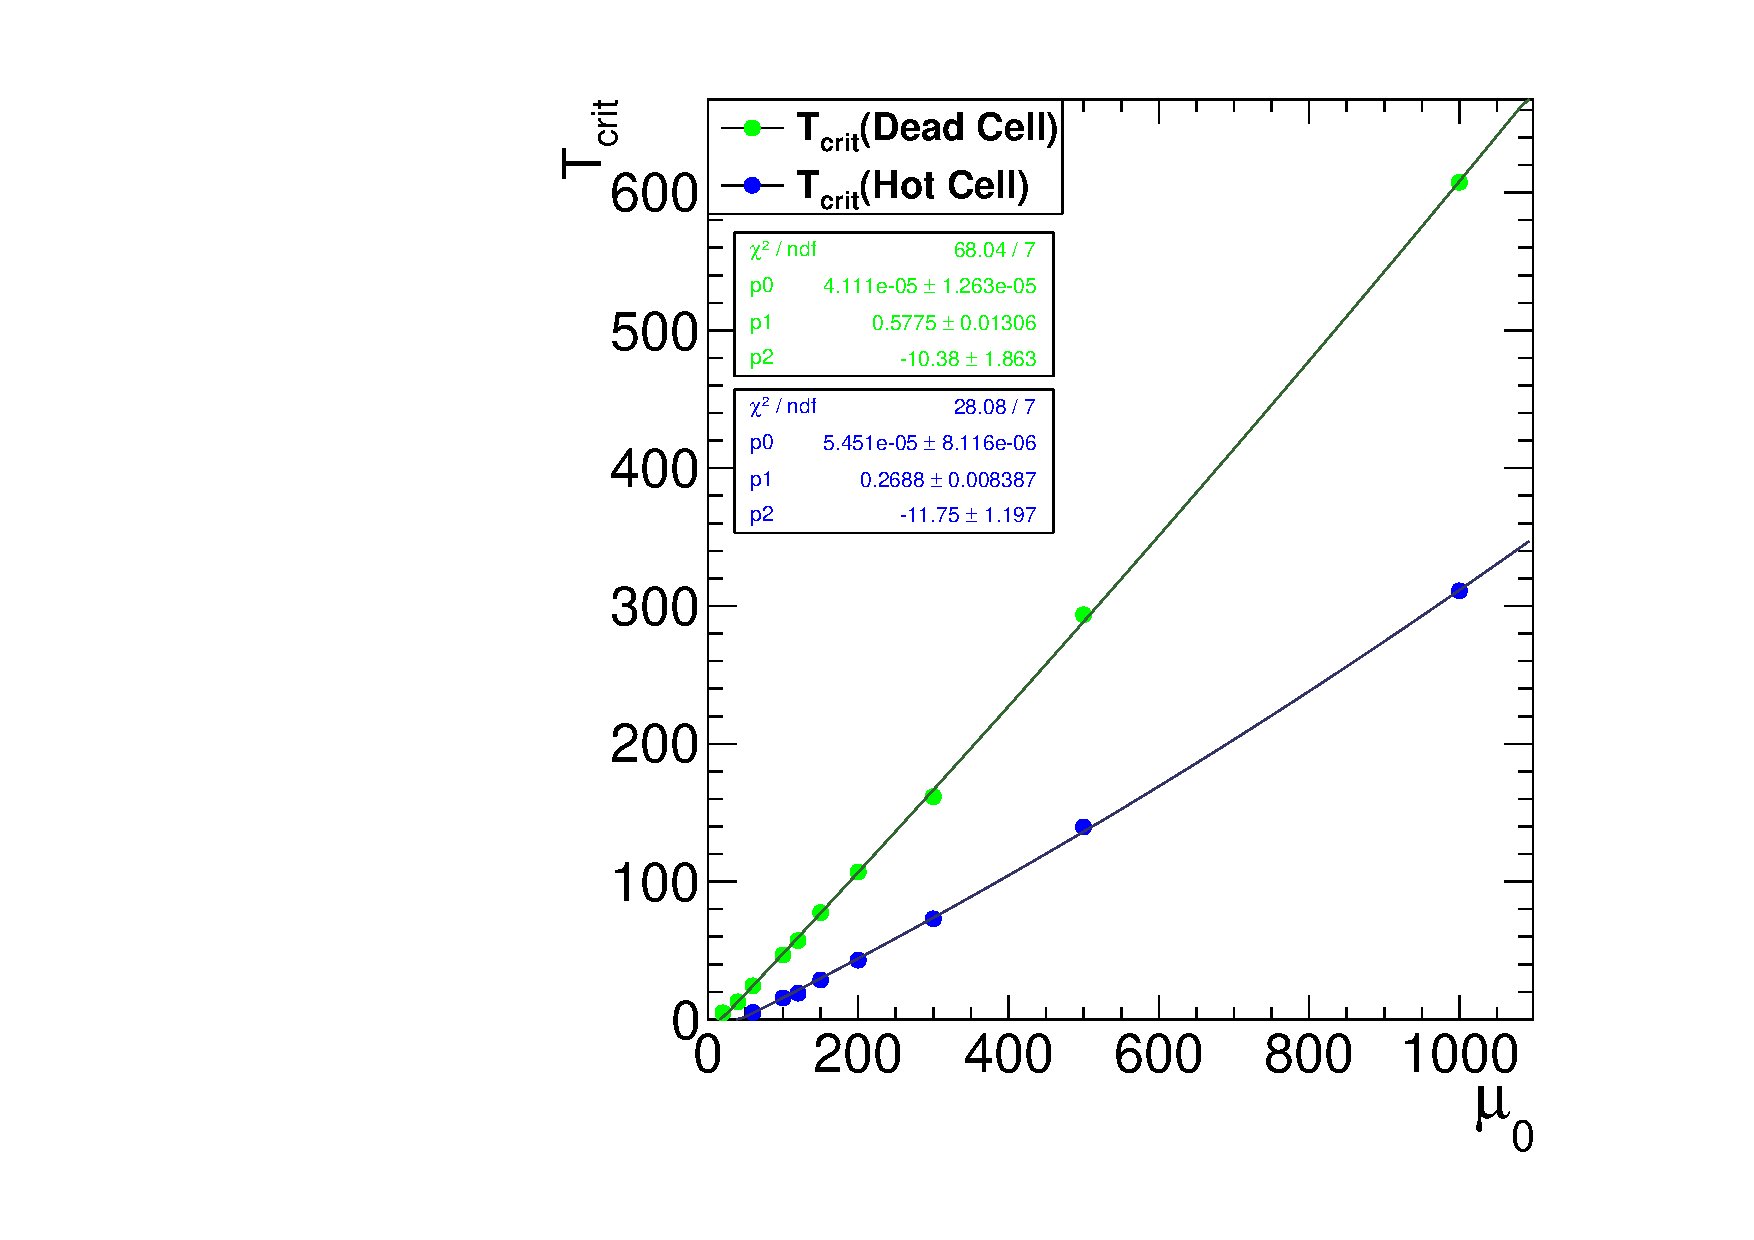
\includegraphics[width=0.55\textwidth]{Chapter03/L1TOnline/Images/L1TOccupancy_TCrit.pdf}
\caption{Graphic showing the results of the determination of $T_{\text{crit}}$ as a function of $\mu_0$ and the corresponding fit for each bad cell hypothesis. Results are for an efficiency of $99\%$ and a fake rate of $1\%$.}
\label{FIGURE:TechnicalWork_L1TOccupancyTCrit}
\end{figure}

To determine the minimum $\mu_0$ and a function of the number of bins we need to fulfil both efficiency and fake rate conditions, this can also be determined with the help of \gls{MC}. Searches for $mu_{min}$ was preformed using an histograms with a predefined number of cells. For each tested $mu_{0}$, five hundred experiments where made by filling all cells with a Poisoning random numbers around $\mu_0$. Resulting cells where then tested with $T$ against the critical value determined for that specific $\mu_0$. The fake rate will be the fraction of experiments where one or more cells are marked as bad. The procedure is repeated for different $mu_{0}$ until the minimum value for this variable is found that exhibits a fake rate of 0.01 or lower. The procedure was repeated for the number of cells of all histograms to be initial monitored by this tool. The obtained values of $\mu_0^{min}$ were fitted with a logarithm function as showed in equation \ref{EQUATION:TechnicalWork_Occupancy_MuMinFits}.

\begin{equation}
\mu_{0}^{min}= a \cdot \ln(b \cdot n_{\text{Bins}} + c) + d
\label{EQUATION:TechnicalWork_Occupancy_MuMinFits}
\end{equation}

On figure \ref{FIGURE:TechnicalWork_L1TOccupancyMuMin}, all the calculated $\mu_0^{min}$ values and the corresponding fits for both bad cell hypotheses tests are showed.

\begin{figure}[!htb]
\centering
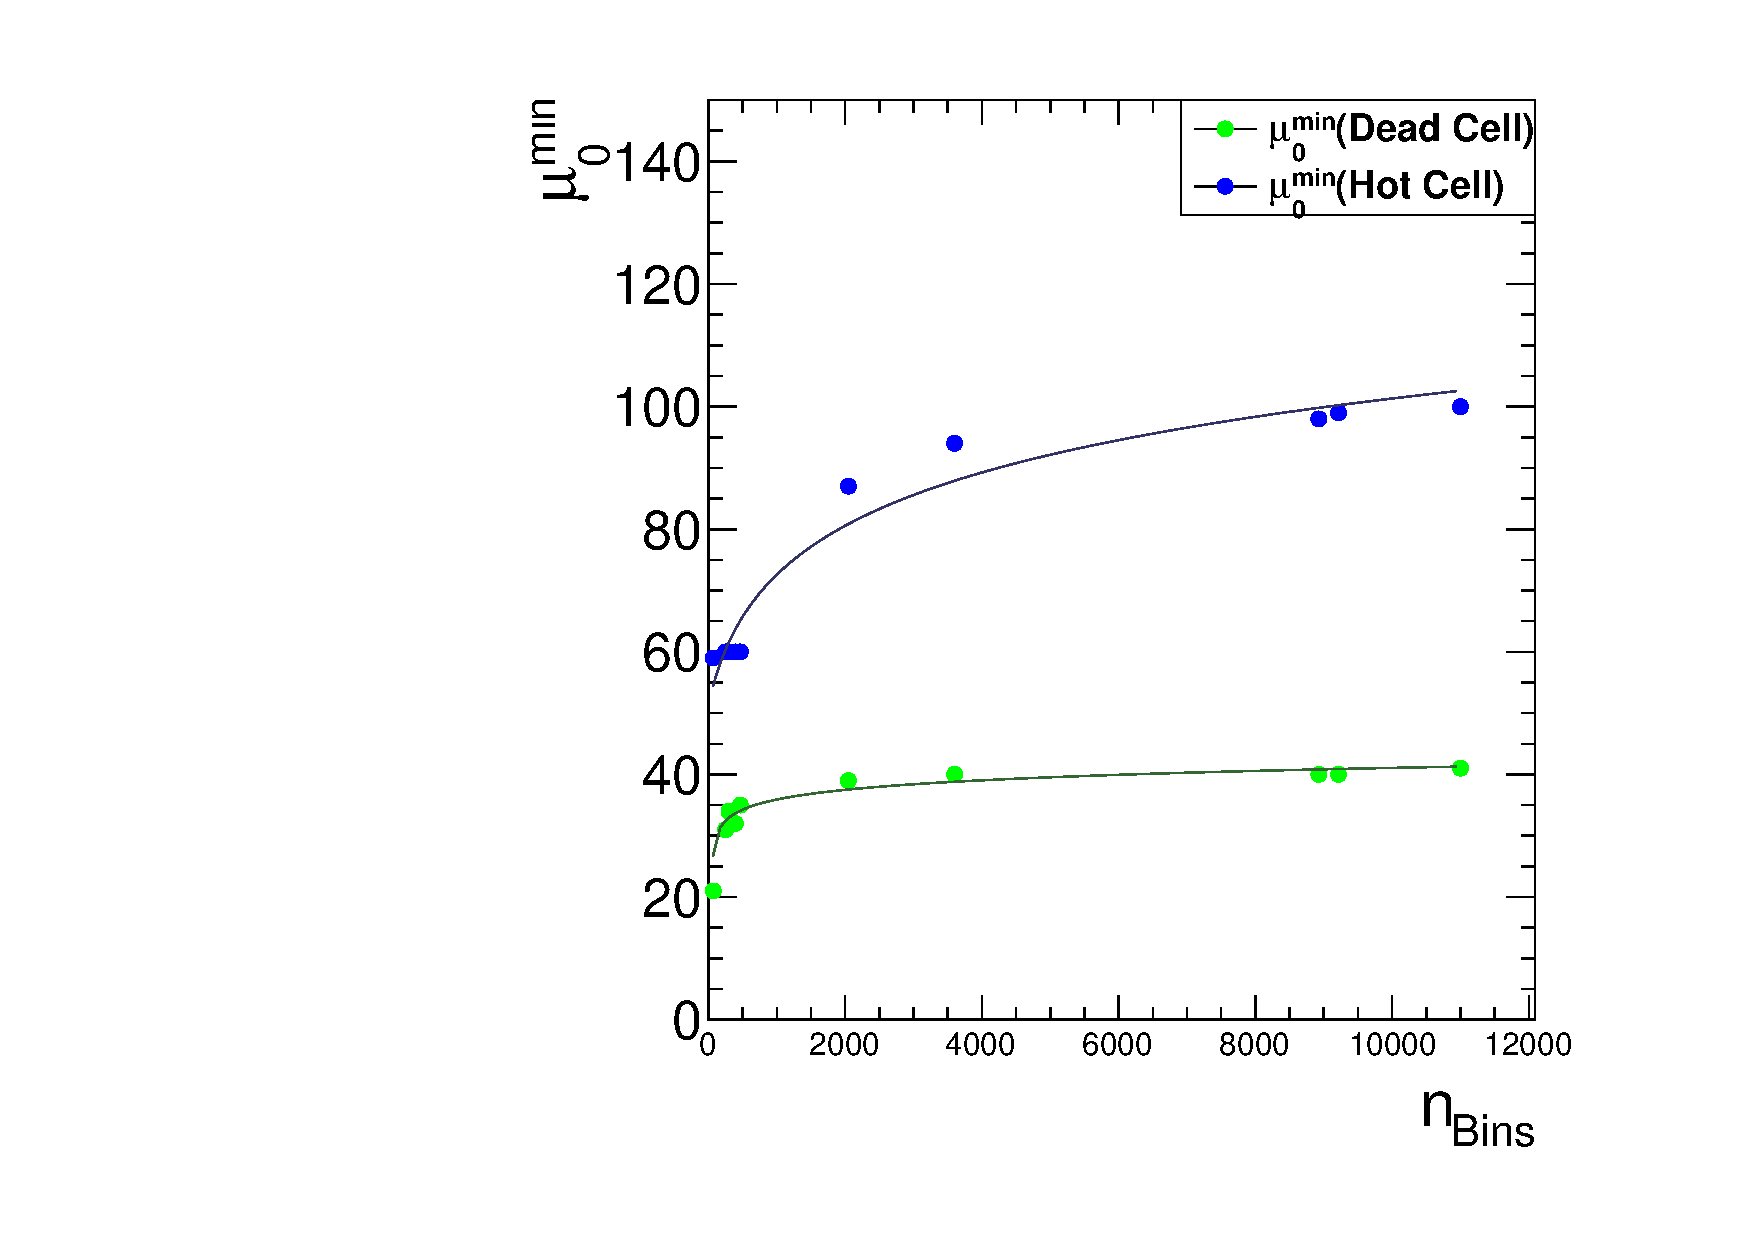
\includegraphics[width=0.55\textwidth]{Chapter03/L1TOnline/Images/L1TOccupancy_MuMin.pdf}
\caption{Graphic showing the results of $\mu_0^{min}$ as a function of the number of bins and the corresponding fit for each bad cell hypothesis. Results are for an efficiency of $99\%$ with a fake rate of $1\%$.}
\label{FIGURE:TechnicalWork_L1TOccupancyMuMin}
\end{figure}

%%%%%%%%%%%%%%%%%%%%%%%%%%%%%%%%%%%%%%%%%%%%%%%%%%%%%%%%%%%%%%%%%%%%%%%%%%%%%%%%%%%%%%%
%%% SUBSUBSECTION
%%%%%%%%%%%%%%%%%%%%%%%%%%%%%%%%%%%%%%%%%%%%%%%%%%%%%%%%%%%%%%%%%%%%%%%%%%%%%%%%%%%%%%%
\subsubsection{Implemented monitoring tool}

% Status: DONE (reviewed J.Pela x1)

The \gls{L1T} occupancy monitor integrates the histograms in blocks of luminosity sections to ensure they have enough statistics. At the end of each luminosity section, with the help of the fits obtained in the previously, each strip of cell median is tested against the histograms $\mu_0^{min}$ for both bad cell hypothesis tests. Cell and strips that are masked are ignored. If all strips have enough statistics the bad cell tests are performed and all cells that fail are marked as bad for the period of integration of the histogram. An exampled of an histograms integrated for a few luminosity sections and the results of the bad cell search are showed in figure \ref{FIGURE:TechnicalWork_L1TOccupancyTests}. 

\begin{figure}[!htb]
\centering
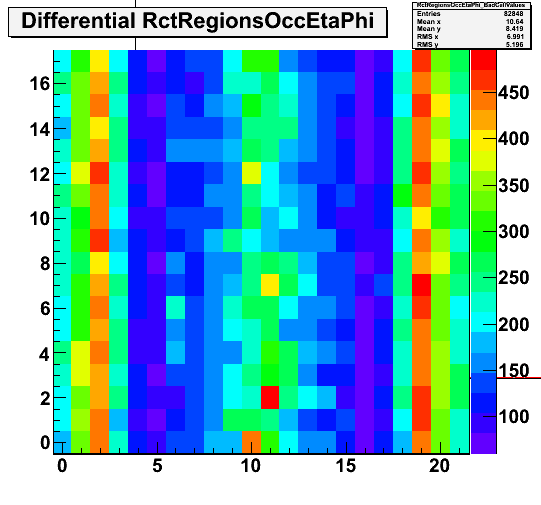
\includegraphics[width=0.45\textwidth]{Chapter03/L1TOnline/Images/L1TOccupancy_Diff.png}
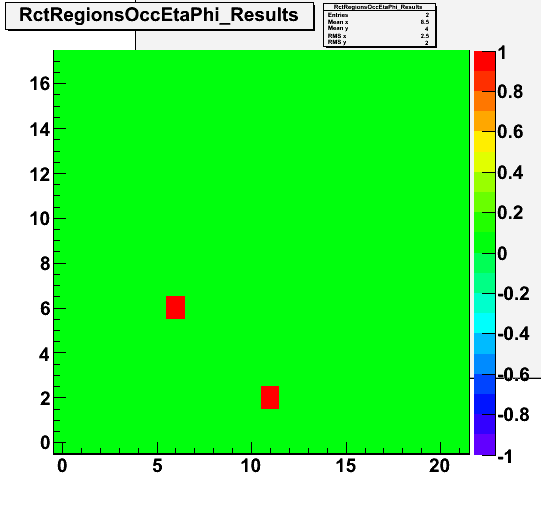
\includegraphics[width=0.45\textwidth]{Chapter03/L1TOnline/Images/L1TOccupancy_Results.png}
\caption{Monitoring plot produced by the \gls{L1T} occupancy monitoring tool for run 207099 while testing \gls{GCT} plot for isolated \gls{EM} region occupancy in $\eta-\phi$. On the left is the histogram under test which have been integrated for enough luminosity sections for meaningful results. On the right is an histogram where the cells that have passed the test are marked in green and red for the cells that failed. Two cells were found that fail the preformed tests.}
\label{FIGURE:TechnicalWork_L1TOccupancyTests}
\end{figure}

An additional plot is produced for each one of the monitored histograms showing the fraction of unmasked cells that pass both bad cell tests. Automatic tests are attached to this histograms and are configured to flag as bad the luminosity sections that show more than 30\% bad cells. This value is too high but was set in order to allow testing the full implementation of the tool and not to flag luminosity sections as bad while some of the original plots need intervention by the subsystem experts.

%%%%%%%%%%%%%%%%%%%%%%%%%%%%%%%%%%%%%%%%%%%%%%%%%%%%%%%%%%%%%%%%%%%%%%%%%%%%%%%%%%%%%%%
%%% SECTION
%%%%%%%%%%%%%%%%%%%%%%%%%%%%%%%%%%%%%%%%%%%%%%%%%%%%%%%%%%%%%%%%%%%%%%%%%%%%%%%%%%%%%%%
\section{Tests Summary}

% Status: DONE (reviewed J.Pela x1)

To simplify the task of the shift crew and certification for physics analysis an tests summary application was developed. This tool collects the results of other tests and presents them in a single set of plots as a function of the luminosity section. Three plots are produced, summaries of the \gls{L1T} rates and \gls{L1T} synchronization monitoring tools, and a global tests summary. In each histogram, the bottom horizontal line is the summary of the lines above, which is marked as bad (red) if any of the tests above fails. This scheme allows the user to quickly identify a problem by back tracing information from what tests where marked as bad starting from the summary line on the \textit{L1T Tests Summary} histogram. An example of plots produced by this application can be found in figure \ref{FIGURE:TechnicalWork_TestsSummary}.

\begin{figure}[!htp]%
\centering
\subfloat[]{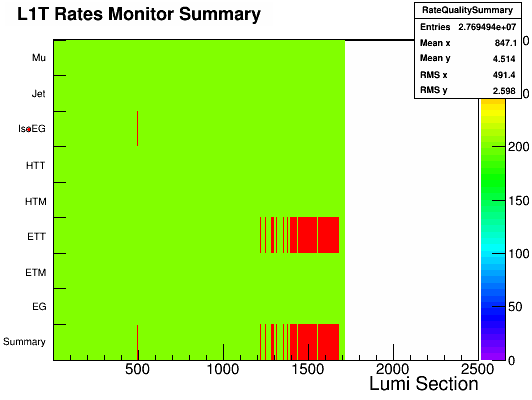
\includegraphics[width=0.45\linewidth]{Chapter03/L1TOnline/Images/RateQualitySummary.png}}\qquad
\subfloat[]{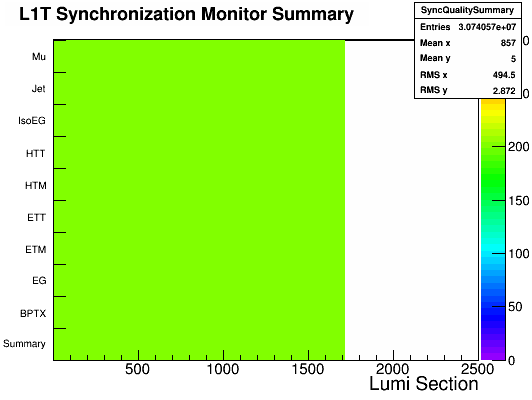
\includegraphics[width=0.45\linewidth]{Chapter03/L1TOnline/Images/SyncQualitySummary.png}}\\
\subfloat[]{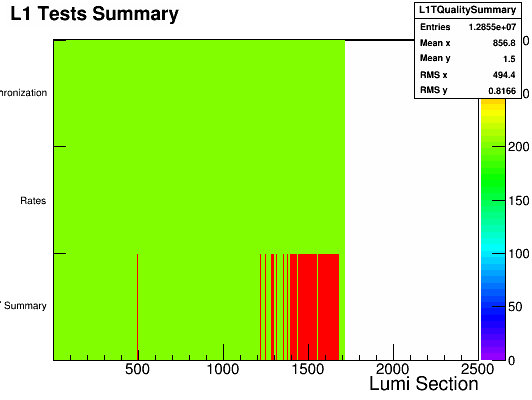
\includegraphics[width=0.45\linewidth]{Chapter03/L1TOnline/Images/L1TQualitySummary.png}}
\caption[Example of the plots produced by the \gls{L1T} test summary monitor]{Example of the plots produced by the \gls{L1T} test summary monitor. Figure (a) summary of all tests made by \gls{L1T} rates monitor. Figure (b) summary of all tests made by \gls{L1T} synchronization monitor, Figure (c) global summary of all tests performed.}
\label{FIGURE:TechnicalWork_TestsSummary}
\end{figure}

The \gls{L1T} occupancy monitoring was executed over histograms produced by other developers. Some of this histograms suffered from pathological problems that needs intervention from their authors. This caused the summary from that monitoring tool to always be flagged as bad. Although implemented, in order to avoid confusion it was decided to not enable this summary plot or add its results to the global summary until necessary changes to the original histograms are made.
